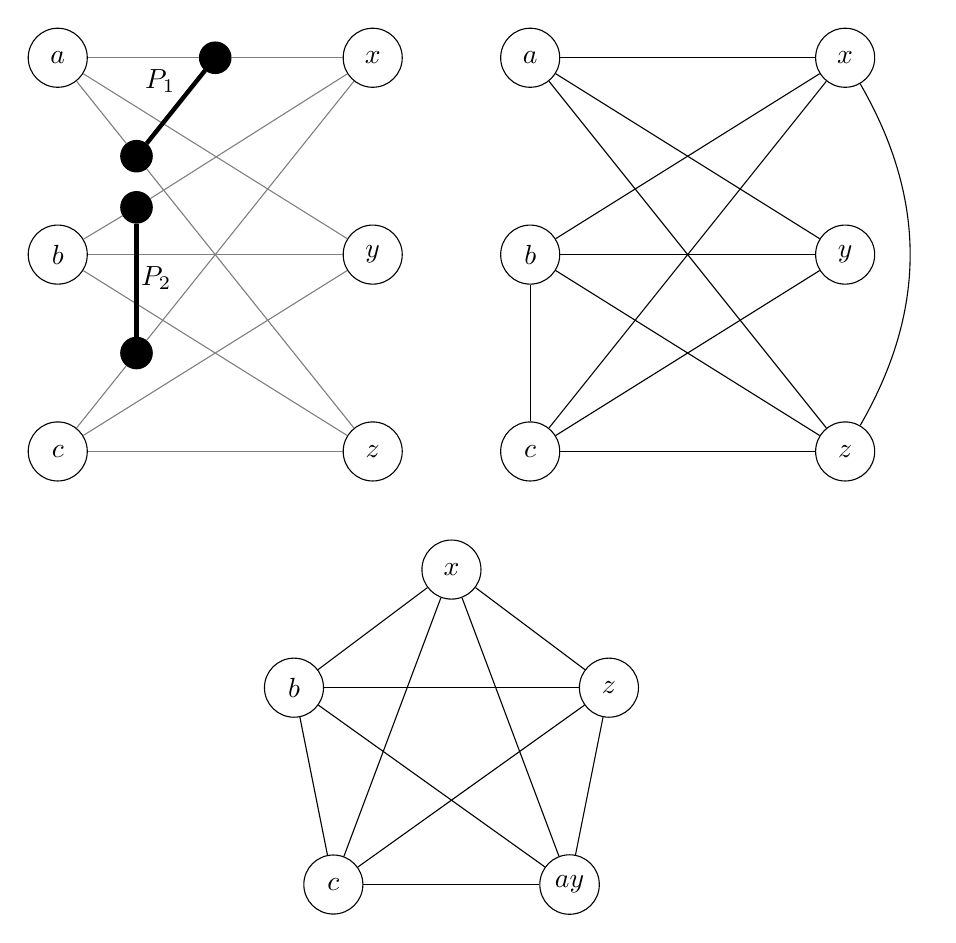
\begin{tikzpicture}
\node [circle, minimum height=0.75cm, draw] (a) at (0,0) {$a$};
\node [circle, minimum height=0.75cm, draw] (b) at (0,-2.5) {$b$};
\node [circle, minimum height=0.75cm, draw] (c) at (0,-5) {$c$};
\node [circle, minimum height=0.75cm, draw] (x) at (4,0) {$x$};
\node [circle, minimum height=0.75cm, draw] (y) at (4,-2.5) {$y$};
\node [circle, minimum height=0.75cm, draw] (z) at (4,-5) {$z$};

\node [circle, minimum height=0.4cm, fill=black, draw] (u1) at (2,0) {};
\node [circle, minimum height=0.4cm, fill=black, draw] (v1) at (1,-1.25) {};
\node [circle, minimum height=0.4cm, fill=black, draw] (u2) at (1,-1.9) {};
\node [circle, minimum height=0.4cm, fill=black, draw] (v2) at (1,-3.75) {};

\draw [color=gray] (a) edge (u1);
\draw [color=gray] (u1) edge (x);
\draw [color=gray] (a) edge (y);
\draw [color=gray] (a) edge (v1);
\draw [color=gray] (v1) edge (z);
\draw [color=gray] (b) edge (u2);
\draw [color=gray] (u2) edge (x);
\draw [color=gray] (b) edge (y);
\draw [color=gray] (b) edge (z);
\draw [color=gray] (c) edge (v2);
\draw [color=gray] (v2) edge (x);
\draw [color=gray] (c) edge (y);
\draw [color=gray] (c) edge (z);

\draw [ultra thick] (u1) edge (v1);
\draw [ultra thick] (u2) edge (v2);

\node at (1.3,-0.3) {$P_1$};
\node at (1.25,-2.8) {$P_2$};

\node [circle, minimum height=0.75cm, draw] (v1) at (6,0) {$a$};
\node [circle, minimum height=0.75cm, draw] (v6) at (6,-2.5) {$b$};
\node [circle, minimum height=0.75cm, draw] (v7) at (6,-5) {$c$};
\node [circle, minimum height=0.75cm, draw] (v3) at (10,0) {$x$};
\node [circle, minimum height=0.75cm, draw] (v4) at (10,-2.5) {$y$};
\node [circle, minimum height=0.75cm, draw] (v5) at (10,-5) {$z$};
\draw  (v1) edge (v3);
\draw  (v1) edge (v4);
\draw  (v1) edge (v5);
\draw  (v6) edge (v3);
\draw  (v6) edge (v4);
\draw  (v6) edge (v5);
\draw  (v7) edge (v3);
\draw  (v7) edge (v4);
\draw  (v7) edge (v5);
\draw  (v6) edge (v7);
\draw [bend left] (v3) edge (v5);

\node [circle, minimum height=0.75cm, draw] (v8) at (5,-6.5) {$x$};
\node [circle, minimum height=0.75cm, draw] (v12) at (3,-8) {$b$};
\node [circle, minimum height=0.75cm, draw] (v11) at (3.5,-10.5) {$c$};
\node [circle, minimum height=0.75cm, draw] (v10) at (6.5,-10.5) {$ay$};
\node [circle, minimum height=0.75cm, draw] (v9) at (7,-8) {$z$};
\draw  (v8) edge (v9);
\draw  (v9) edge (v10);
\draw  (v10) edge (v11);
\draw  (v11) edge (v12);
\draw  (v12) edge (v8);
\draw  (v8) edge (v10);
\draw  (v10) edge (v12);
\draw  (v12) edge (v9);
\draw  (v9) edge (v11);
\draw  (v11) edge (v8);
\end{tikzpicture}